\section{Filter Fission}

This section covers an improved form of fission applied to nodes of the
general graph.  Applying fission to nodes of the general graph allows
the compiler to express more precise communication patterns for the
distribution of input items to the fission products.  This allows the
fission technique to avoid unnecessary duplication (and thus
communication) of input items.  Figure~\ref{fig:fission-versus}
demonstrates an example of the savings in communication for fission on
the general graph versus fission on the StreamIt graph.

A key design goal for the implementation of fission on the general graph
was that communication between levels of the stream graph be efficient
(see Section~\ref{sec:levels} for the description of a level).  Often
when data parallelism is applied, the producer filters in level $l$ are
fissed at the same width as the consumer filters in level $l + 1$.  To
make this common case efficient, general graph fission communicates a
large number of items between disjoint producer-consumer pairs from the
levels.  Next, a small number of items (the number of items inspected by
the consumer filter) is duplicated and communicated from consumer to a
producer in a different pair.  Figure~\ref{fig:fission-versus}(c),
demonstrates this pattern, with $u_i$ and $v_i$ forming the pairs.  Each
pair should be mapped to the same core, so that the bulk of
communication for the fission distribution pattern is intra-core.  For
Figure~\ref{fig:fission-versus}(c), if the pairs are mapped to same
core, only 3 of 12 items are communicated inter-core.


In the general case, when fissing a filter that peeks, i.e., a filter
$f$ with $e(W, f) - o(W, f) = \mt{dup}_f < C(f) > 0$, by $P$, the producers
of $f$ need to duplicate output items to an average of:

\[ \max \left ( 1 + \frac{C(f)}{M(S, f) \cdot o(W, f) / P}, P \right )\]

\noindent fission products of $f$.  Figure~\ref{fig:fission-sharing}
gives an example of the required sharing for a fission application.
The filter $f$ is duplicated 4 ways, has $C(f) = 9$, $o(W, F) = 4$,
and $M(S, f) = 16$.  From the above formula, each item is duplicated
to an average of $3.25$ fission products.

Before we describe the fission transformation, we need to list the
preconditions that must hold before fission of $f$ by $P$ in the general
graph can be performed:
\begin{itemize}
\item $C(f) < (M(S,f) / P) \cdot o(W, f)$. The items remaining of
  the input buffer of the original filter after initialization must be
  less than the number of items dequeued by each fission product.
  This implies $\mt{dup}_f < (M(S,f) / P) \cdot o(W, f)$ since
  $\mt{dup}_f \le C(f)$.  If $\mt{dup}_f$ for the steady-state is greater
  than the number of items that each fission product pops, then some
  items will be duplicated to more than 2 fission products.  We do not
  support this case, as it can be avoided, and we want to limit
  inter-core communication.

\item $M(S,f) \mod P = 0$. In this version of the algorithm we create
  fission products with equal work, an equal division of the original
  steady-state multiplicity of $f$.  This restriction can be relaxed
  via simple modifications to the algorithm.
\end{itemize}
\noindent All the multiplicities of the steady-state can be multiplied
by the same constant $c$, and the result will still be a valid
steady-state.  We call this process {\it increasing} the steady-state
of the graph by $c$.  Each of these preconditions can be enforced by
increasing the steady-state of the graph.


\begin{figure*}
\centering
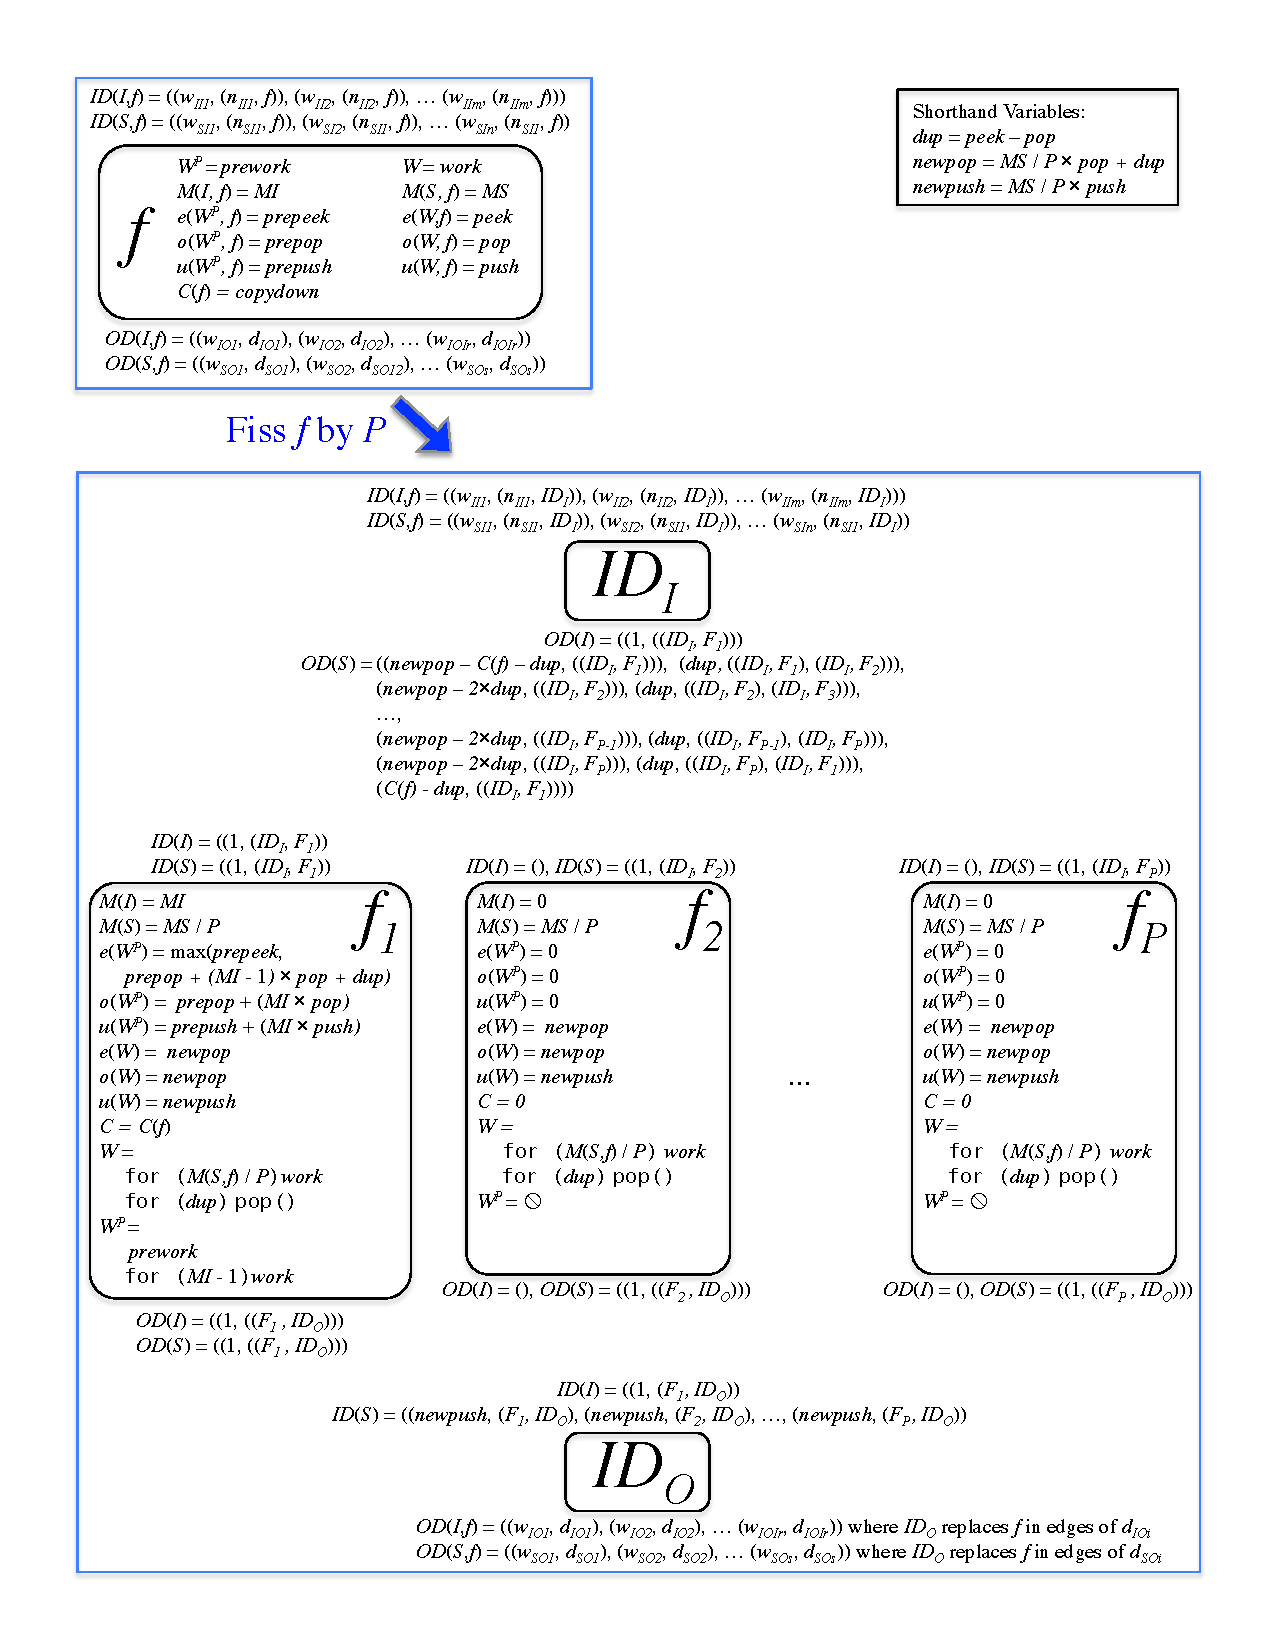
\includegraphics[width=\textwidth]{figures/general-fission.pdf}
\caption[Fission of a node in the general stream graph.]{Fission of a
  node $f$ by $P$ in the general stream
  graph.\label{fig:general-fission}}
\end{figure*}

The details of fission on a filter of the general stream graph are
given in Figure~\ref{fig:general-fission}.  The process includes the
following steps (Figure~\ref{fig:general-fission} illustrates steps
1-9): 
\begin{enumerate}
\item Create $P$ copies of $f$ and set their rates
and work functions according to Figure~\ref{fig:general-fission}.
\item Create two identity nodes, $ID_I$ and $ID_O$, that will encode
  the distribution for the fission.
\item Move the initialization stage computation of $f$ to $f_1$
  according to Figure~\ref{fig:general-fission}. 
\item Move input distribution of $f$ to $ID_I$
replacing occurrences of $f$ with $ID_I$ in edges.
\item Move output distribution of $f$ to $ID_O$, replacing
occurrences of $f$ with $ID_O$ in edges.
\item Create the fission duplication pattern in the
output distribution of $ID_I$.
\item Create a round robin joining pattern for the output identity
  filter $ID_O$ to receive from each fission product.
\item For each node $p$ that is a producer of $f$, replace the
 occurrences of $f$ with $O_I$ in the edges of the dupsets of $p$'s
 output distribution.
\item For each node $c$ that is a consumer of $f$, replace the
 occurrences of $f$ with $O_O$ in incoming edges $c$'s input
 distribution.
\item \textsc{SynchRemove}($ID_I$)
\item \textsc{SynchRemove}($ID_O$)
\end{enumerate}

To understand the transformation, we first need to understand the item
distribution and sharing that is required by fission on a filter $f$
that adheres to the preconditions above.
Figure~\ref{fig:fission-sharing2} gives another example of the input
items required by fission products.  In this example, both:

\[ C(f) = \mt{dup}_f < (M(S,f) / p) \cdot o(W, f) \]
\[ M(S, f) \mod P = 0\]

\noindent so $f$ adheres to the preconditions stipulated above for
general fission.  In the example, the items read for $f$ plus its
fission products for $P=4$ are shown for the initialization plus two
steady-states.  After the initialization stage, $C(f) = 2$ items are
enqueued to the input buffer by the producer(s) to $f$, and $M(S,f)
\cdot o(W, f) = 16$ items are enqueued by the producer(s) for each
steady-state.  Examining the sharing requirement for fission products of
the second steady-state, we can see a pattern emerge with the following
features:

\begin{itemize}
\item No item is read by more than 2 fission products.
\item  A fission product does not need to remember items across
  steady-state executions of itself.
\item Only the first fission product $f_1$ is required to receive the $C(f)$
  initialization  items because $C(F) < (M(S,f) / p) \cdot o(W, f)$,
  and it will consume the $C(f)$ items on its first invocation.
\item The presence of the $C(f)$ items in the input buffer after
  initialization must be accounted for by shifting the read pattern
  for the fission products.  The first fission product $f_1$ is offset by
  $C(f)$ items in that it reads its first $C(f)$ items from the
  previous execution stage.  In the steady-state, $f_1$ executing at
  steady-state iteration $i$ shares items with $f_P$ executing at
  steady-state iteration $i-1$.
\end{itemize}


\begin{figure*}
\centering
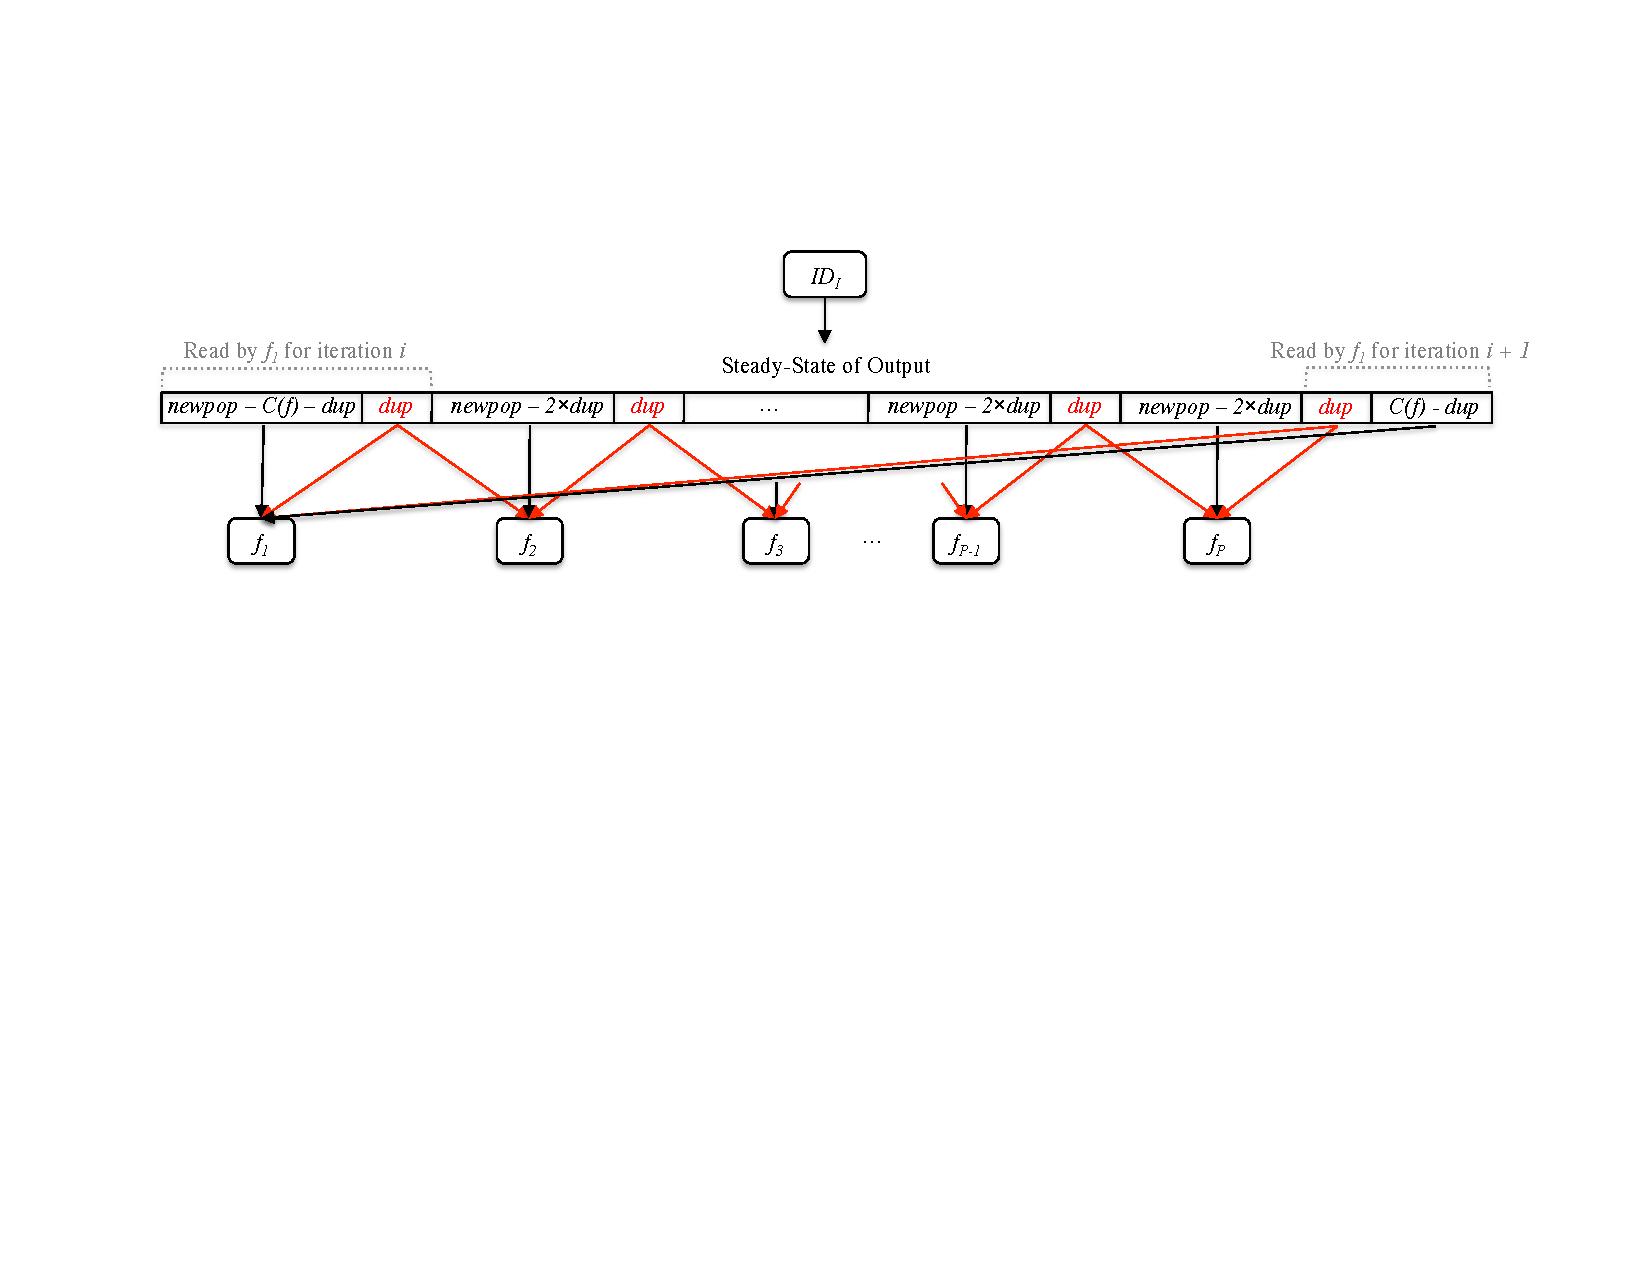
\includegraphics[width=\textwidth]{figures/split-pattern.pdf}
\caption[The output distribution required for general
fission.]{
The steady-state output distribution installed for identity node
$ID_I$ by general fission.  Red edges denote items that are shared
across fission products via duplication.  Though not demonstrated in
the example of Figure~\ref{fig:fission-sharing2}, in the general
case, if $C(f) > dup$, $C(f) - dup$ items at the end of the
steady-state input are distributed to $f_1$. \label{fig:split-pattern}}
\end{figure*}

The general fission transformation creates two identity nodes ($ID_I$
and $ID_O$) that are encoded to implemented the data distribution for
the fission products.  The pattern seen in
Figure~\ref{fig:fission-sharing2} and described above is common to the
transformation for all filters we seek to fiss that meet the
preconditions of the transformation.  This sharing pattern is encoded
in the output distribution pattern for the identity filter $ID_I$.
Figure~\ref{fig:split-pattern} shows the weights for the output
distribution and how these weights are distributed to the fission
products.

The input distribution of $ID_I$ is set to the input distribution of
$f$.  Thus, $ID_I$ joins data as described by $f$'s input
distribution, and splits data according to the fission output pattern
for sharing between at most 2 filters.  The output identity $ID_O$
collects the output items of the fission products in a weighted round
robin, and the distributes them according to $f$'s output distribution.

Since a fission product, does not need to remember items across
firing, a fission product's peek rate equals its pop rate in the
steady-state.  This rate equals the division of $f$'s dequeued
items plus the number of items inspected but not dequeued by $f$ for
each firing:   

\[ o(S,f_i) = e(S, f_i) = \frac{M(S, f)}{P} \cdot o(W, f) + \mt{dup} \]

\noindent The peeking of the original filter $f$ is now encoded in
the sharing across fission products achieved via the duplication
pattern.

The computation and communication performed by $f$ during the
initialization stage is transferred completely to the first fission
product, $f_1$.  Since, by construction, only $f_1$ requires the items
remaining after the initialization stage.  The other fission products
are idle during this stage.

The final steps of the general fission transformation applies
\textsc{SynchRemove} to remove the identity filters, and stitch the
communication directly between the fission products and $f$'s
producer(s) and consumer(s).
